\documentclass{beamer}

\usepackage[utf8]{inputenc}
\usepackage[T1]{fontenc}
\usepackage{tikz}
\usetikzlibrary{shadows}
\usepackage{lmodern}
\usepackage{mathrsfs}
\usepackage{mathabx}

\setbeamercolor{upcol}{fg=black,bg=black!40}
\setbeamercolor{lowcol}{fg=black,bg=black!20}

\setbeamertemplate{navigation symbols}{}
\usefonttheme[onlymath]{serif}
\setbeamertemplate{blocks}[rounded][shadow=true,upper=upcol,lower=lowcol]

\pgfdeclareimage[height=1cm]{rex}{rex128.pdf}
\logo{\pgfuseimage{rex}}

\DeclareMathOperator{\dist}{\mathrm{dist}}
\DeclareMathOperator{\sign}{\mathrm{sign}}
\DeclareMathOperator{\spn}{\mathrm{span}}

\newcommand{\todo}[1]{
	\begin{beamerboxesrounded}[upper=upcol,lower=lowcol,shadow=true]{ToDo}
	#1
	\end{beamerboxesrounded}	
}

\author{Tomáš Kalvoda \\ \texttt{tomas.kalvoda@fit.cvut.cz}}
\title{Nonlinear classification: Support Vector Machines}
\subtitle{COW\&MP, Dolní lomná}
\date{May 24, 2013}
\institute{KAM FIT ČVUT}

<% slide = 0; slides = 23 %>

%%%%%%%%%%%%%%%%%%%%%%%%%%%%%%%%%%
%% Begin Document
%%%%%%%%%%%%%%%%%%%%%%%%%%%%%%%%%%
\begin{document}

<%= rex(slide,slides) %>
<% slide += 1 %>
\begin{frame}
	\titlepage
\end{frame}

<%= rex(slide,slides) %>
<% slide += 1 %>
\begin{frame}[c]
	\frametitle{Classification problem (2 classes)}
	\begin{columns}[t]
		\column<1->{.5\textwidth}
			Linear classification

			\bigskip\bigskip
			\begin{tikzpicture}[scale=1.2]
				<% w = -0.6; b = 0.3; bp = 0.2; bm = -0.5; n = 25 %>
				\def\w{<%= w %>}
				\def\b{<%= b %>}
				\def\bp{<%= bp %>}
				\def\bm{<%= bm %>}
				% samples of y=1 class
				<% n.times do %>
					<% x = rand(-1.8..1.8); y = rand(0..1.8) %>
					<% if y > w * x + bp %>
						\draw[blue,fill=blue] (<%= x %>, <%= y %>) circle (1pt);
					<% end %>
				<% end %>

				% samples of y=-1 class
				<% n.times do %>
					<% x = rand(-1.8..1.8); y = rand(-1.8..0) %>
					<% if y < w * x + bm %>
						\draw[green,fill=green] (<%= x %>, <%= y %>) circle (1pt);
					<% end %>
				<% end %>
				\draw[red,dashed,domain=-2:2,thick] plot (\x,{\w*\x+(\bp+\bm)/2});
			\end{tikzpicture}
		\column<2>{.5\textwidth}
			Nonlinear classification

			\bigskip\bigskip
			\begin{tikzpicture}[scale=1.2]
				<% n = 50; fac = 0.7; eps = 0.1 %>
				\def\fac{<%= fac %>}
				% samples of y=1 class
				<% n.times do %>
					<% x = rand(-1.9..1.9); y = rand(0.0..3.0) %>
					<% if y > fac * Math.sqrt(4-x*x) + eps %>
						\draw[blue,fill=blue] (<%= x %>, <%= y %>) circle (1pt);
					<% end %>
				<% end %>

				% samples of y=-1 class
				<% n.times do %>
					<% x = rand(-1.9..1.9); y = rand(0.0..3.0) %>
					<% if y < fac * Math.sqrt(4-x*x) - eps %>
						\draw[green,fill=green] (<%= x %>, <%= y %>) circle (1pt);
					<% end %>
				<% end %>
				\draw[red,dashed,domain=-1.9:1.9,thick,samples=50] plot (\x,{\fac*sqrt(4-\x*\x)});
			\end{tikzpicture}
	\end{columns}
\end{frame}

<%= rex(slide,slides) %>
<% slide += 1 %>
\begin{frame}[c]\frametitle{Applications of SVM (90s, [Vapnik, 1979])}
	\begin{itemize}
		\item Isolated handwritten digit recognition.
		\vfill
		\item Object recognition.
		\vfill
		\item Speaker identification.
		\vfill
		\item Face detection in images.
	\end{itemize}
\end{frame}

<%= rex(slide,slides) %>
<% slide += 1 %>
\begin{frame}[c]\frametitle{Setup}
	\begin{itemize}
		\item We are given some initial data and their classes:
			\[
				\{(x_i,y_i) \,:\, i=1,2,\ldots,\ell\},
			\]
			where $x_i \in \mathbb{R}^d$, $y_i \in \{-1,1\}$ for any $i=1,2,\ldots,\ell$.
		\vfill
		\item Our task: For $x\in\mathbb{R}^d$ decide whether it belongs to $y=1$ or $y=-1$ class.
	\end{itemize}
\end{frame}

%%%%%%%%%%%%%%%%%%%%%%%%%%%%%%%%%%
%% Separable case
%%%%%%%%%%%%%%%%%%%%%%%%%%%%%%%%%%
\section{Linear case}
\label{sec:linear_case}

<%= rex(slide,slides) %>
<% slide += 1 %>
\begin{frame}[t]\frametitle{Linear SVM}

	{\centering
		\begin{tikzpicture}[
			domain=-2:2,
			scale=1.5
		]
		<% w = -0.6; b = 0.3; bp = 1.2; bm = -0.4; n = 25; eps=0.2 %>
		\def\w{<%= w %>}
		\def\b{<%= b %>}
		\def\bp{<%= bp %>}
		\def\bm{<%= bm %>}
		\begin{scope}
			\clip (-2,-2) rectangle (2,2);
			\uncover<1>{
				\draw[thick,red] plot (\x,{\w*\x+\b+.3});
			}
			\uncover<2->{
				\draw[thick,red] plot (\x,{\w*\x+\b});
				\draw[thick,red!60,dashed] plot (\x,{\w*\x+\bp});
				\draw[thick,red!60,dashed] plot (\x,{\w*\x+\bm});
			}
		\end{scope}
		% annotation
		% R^d
		\draw[thick,->] (-2.2,0) -- (-1.8,0);
		\draw[thick,->] (-2.2,0) -- (-2.2,.4);
		\node at (-2.2,0) [anchor=south west] {$\mathbb{R}^d$};

		% hyper planes
		\uncover<1>{
			\node at (2,{\w*2+\b+.3}) [right] {$H:\, w\cdot x + b = 0$};
		}
		\uncover<2->{
			\node at (2,{\w*2+\b}) [right] {$H_0:\, w\cdot x + b = 0$};
			\node at (2,{\w*2+\bp}) [right] {$H_+:\, w\cdot x + b = 1$};
			\node at (2,{\w*2+\bm}) [right] {$H_-:\, w\cdot x + b = -1$};
		}

		% normal vectors
		\uncover<1>{
			\draw[black,thick,->] (-1.5,{\w*(-1.5)+\b+.3}) -- node[anchor=south east] {$w$} +({-.6*\w},.6);
		}
		\uncover<2->{
			\draw[black,thick,->] (-1.5,{\w*(-1.5)+\b}) -- node[anchor=south east] {$w$} +({-.6*\w},.6);
		}

		\uncover<3>{
			% gap (a.k.a. margin)
			\pgfmathsetmacro{\fac}{(\bm-\bp)/(1+\w*\w)}
			\draw[black,thick,<->] (-.5,{\w*(-.5)+\bm}) -- node[anchor=south east,fill=white,opacity=.8] {margin (gap)} +(\w*\fac,-\fac);
			\node at (2,1.5) [right] {$\dist(H_+,H_-) = \frac{2}{\|w\|}$};
		}

		% samples of y=1 class
		<% n.times do %>
			<% x = rand(-1.8..1.8); y = rand(0..1.8) %>
			<% if y > w * x + bp + eps %>
				\draw[blue,fill=blue] (<%= x %>, <%= y %>) circle (1pt);
			<% end %>
		<% end %>

		% samples of y=-1 class
		<% n.times do %>
			<% x = rand(-1.8..1.8); y = rand(-1.8..0) %>
			<% if y < w * x + bm - eps %>
				\draw[green,fill=green] (<%= x %>, <%= y %>) circle (1pt);
			<% end %>
		<% end %>

		% support vectors
		<% 2.times do %>
			<% x = rand(-1..1) %>
			\only<1>{
				\draw[fill=blue,draw=blue] (<%= x %>, <%= w * x + bp %>) circle (1pt);
			}
			\only<2->{
				\draw[draw=black,fill=blue] (<%= x %>, <%= w * x + bp %>) circle (1.5pt);
			}			
		<% end %>
		<% x = rand(-1..1) %>
		\only<1>{
			\draw[fill=green,draw=green] (<%= x %>, <%= w * x + bm %>) circle (1pt);
		}
		\only<2->{
			\draw[draw=black,fill=green] (<%= x %>, <%= w * x + bm %>) circle (1.5pt);
		}
		\end{tikzpicture}
	\par}
	\only<1>{
		\vfill
		\begin{align*}
			\text{Assumptions:} \quad \exists w\in\mathbb{R}^d, \, b\in\mathbb{R}: \quad & w \cdot x_i + b > 0, \, y_i = 1 \\
				& w \cdot x_i + b < 0, \, y_i = -1.
		\end{align*}
		\vfill
	}
	\only<2->{
		\vfill
		\begin{align*}
			\text{Equivalently:} \quad \exists w\in\mathbb{R}^d, \, b\in\mathbb{R}: \quad & w \cdot x_i + b \geq 1, \, y_i = 1 \\
				& w \cdot x_i + b \leq -1, \, y_i = -1.
		\end{align*}
		\vfill
	}
\end{frame}

<%= rex(slide,slides) %>
<% slide += 1 %>
\begin{frame}[c]\frametitle{Basic idea of the SVM}
    \begin{block}{Support vectors\ldots}
    	\ldots are those training points $x_i$ that lie on hyperplanes $H_+$ or $H_-$.
    \end{block}
    \vfill
    \begin{block}{Goal:}
    	\emph{Maximize} the margin (gap) between $H_+$ and $H_-$.
    \end{block}
\end{frame}

<%= rex(slide,slides) %>
<% slide += 1 %>
\begin{frame}[c]\frametitle{Primal problem: Summary for the linear separable case}
	\begin{block}{Training data}
		We are given $\ell\in\mathbb{N}$ samples 
		\[
			\big\{ (x_i,y_i) \in \mathbb{R}^d \times \{-1,1\} \,:\, i = 1,2,\ldots,\ell \big\}.
		\]
	\end{block}
	\vfill
	\pause
	\begin{block}{Our task}
		Minimize
		\[
			f: \mathbb{R}^d \times \mathbb{R} \to \mathbb{R}, \quad f(w,b) := \frac{1}{2} \| w\|^2
		\]
		subject to $\ell$ linear inequality constraints
		\[
			g_i(w,b) := y_i ( w \cdot x_i + b) - 1 \geq 0, \quad i = 1,2,\ldots,\ell.
		\]
	\end{block}
	\vfill
	\pause
	\begin{block}{Classification}
		If $w_*$ and $b_*$ solve the problem above then the
		class of $x\in\mathbb{R}^d$ is given by
		\[
			\sign (w_* \cdot x + b_*).
		\]
	\end{block}
\end{frame}

<%= rex(slide,slides) %>
<% slide += 1 %>
\begin{frame}[c]\frametitle{Lagrange formulation}
	\begin{block}{}
		Minimize $f: \mathbb{R}^n \to \mathbb{R}$ subject to $g_i(z) \geq 0$, $g_i: \mathbb{R}^n \to \mathbb{R}$, $1\leq i\leq\ell$.
	\end{block}
	\vfill
	{\centering
		\begin{tikzpicture}
			\draw[thick,->] (-.5,1.5) -- (-.5,-1.5);
			\node at (-.5,0) [left=.5cm,text width=4cm,align=center] {\begin{block}{Necessary}$f,g_i \in C^1$, LICQ \end{block}};
			\draw[thick,->] (.5,-1.5) -- (.5,1.5);
			\node at (.5,0) [right=.5cm,text width=4cm,align=center] {\begin{block}{Sufficient}$f\in C^2$, $g\in C^2$ and
			\[
				v^T \nabla_{\!\!zz}\mathscr{L}(x;\lambda)v \geq 0
			\] for all suitable $v$.\end{block}};
		\end{tikzpicture}
	\par}
	\vfill
	\begin{block}{Karush-Kuhn-Tucker (KKT) Conditions}
		Let $\mathscr{L}(z;\lambda) := f(z) - \lambda^T g(z), \quad z \in \mathbb{R}^n, \, \lambda \in \mathbb{R}^n$.
		\begin{align*}
			\nabla_{\!\!z} \mathscr{L}(z;\lambda) &= 0, & g(z) &\geq 0, \\
			\lambda &\geq 0, & \lambda_i g_i(z) &= 0 \quad i=1,2,\ldots,\ell.
		\end{align*}	
	\end{block}
\end{frame}

<%= rex(slide,slides) %>
<% slide += 1 %>
\begin{frame}[c]{In our case}
	Lagrangian for our particular case is given by
	\[
		\mathscr{L}(w,b;\lambda) = \frac{1}{2}\|w\|^2 - \sum_{i=1}^\ell \lambda_i y_i(w\cdot x_i + b) + \sum_{i=1}^\ell \lambda_i.
	\]
	and KKT conditions are
	\begin{align*}
		w - \sum_{i=1}^\ell \lambda_i y_i x_i &= 0, & \sum_{i=1}^\ell \lambda_i y_i &= 0, \\
		y_i(w\cdot x_i + b) - 1 &\geq 0, & \lambda &\geq 0, \\
		\lambda_i \big( y_i (w \cdot x_i + b) - 1\big) &= 0.
	\end{align*}
	\vfill
	\begin{block}{Note: Quadratic programming problem}
		Objective function is quadratic and convex, constraints are linear.
	\end{block}
\end{frame}

<%= rex(slide,slides) %>
<% slide += 1 %>
\begin{frame}[c]\frametitle{Wolfe dual problem}
	\begin{block}{The problem (P)}
		Minimize $f: \mathbb{R}^n \to \mathbb{R}$ subject to $g_i(z) \geq 0$, where $f$ and $-g_i$ are convex functions.
	\end{block}
	\vfill
	\pause
	\begin{block}{Wolfe dual}
		Maximize $\mathscr{L}(z;\lambda)$ with respect to $z,\lambda\in\mathbb{R}^n$ subject to conditions
		\[
			\nabla_{\!\!z} \mathscr{L}(z;\lambda) = 0 \quad \text{and} \quad \lambda \geq 0.
		\]
	\end{block}
	\vfill
	\pause
	\begin{block}{}
		\begin{itemize}
			\item If $z_* \in \mathbb{R}^n$ solves (P), then it solves the Wolfe dual problem with some $\lambda_* \in \mathbb{R}^n$.
			\item Every local solution $x_*$ to a convex programming problem is a global solution.
		\end{itemize}
	\end{block}
\end{frame}

<%= rex(slide,slides) %>
<% slide += 1 %>
\begin{frame}[c]\frametitle{Wolfe dual: Our problem}
	\begin{block}{Wolfe dual}
		Maximize
		\only<1>{
		\[
			\mathscr{L}(w,b;\lambda) = \frac{1}{2}\|w\|^2 - \sum_{i=1}^\ell \lambda_i y_i (w \cdot x_i + b) + \sum_{i=1}^\ell \lambda_i
		\]
		}
		\only<2>{
		\[
			\mathscr{L}(w,b;\lambda) = \sum_{i=1}^\ell \lambda_i - \frac{1}{2} \sum_{i,j=1}^\ell \lambda_i \lambda_j y_i y_j \, x_i \cdot x_j
		\]
		}
		with respect to $w\in\mathbb{R}^d$, $b \in \mathbb{R}$, and $\lambda\in\mathbb{R}^d$ subject to
		\only<1>{
			\[
				w = \sum_{i=1}^\ell \lambda_i y_i x_i, \quad \sum_{i=1}^\ell \lambda_i y_i = 0, \quad \text{and} \quad \lambda \geq 0.
			\]
		}
		\only<2>{
			\[
				\left( w = \sum_{i=1}^\ell \lambda_i y_i x_i \right), \quad \sum_{i=1}^\ell \lambda_i y_i = 0, \quad \text{and} \quad \lambda \geq 0.
			\]
		}
	\end{block}
\end{frame}

<%= rex(slide,slides) %>
<% slide += 1 %>
\begin{frame}[c]\frametitle{Illustration}
	{\centering
		\only<1>{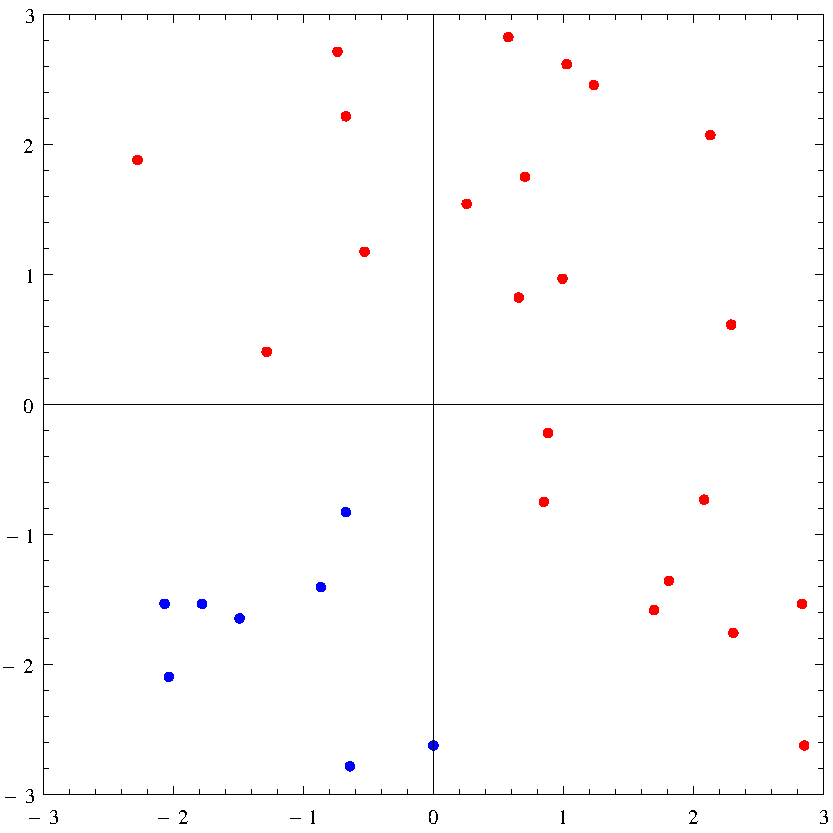
\includegraphics[scale=.55]{figures/math_lin_a}}
		\only<2>{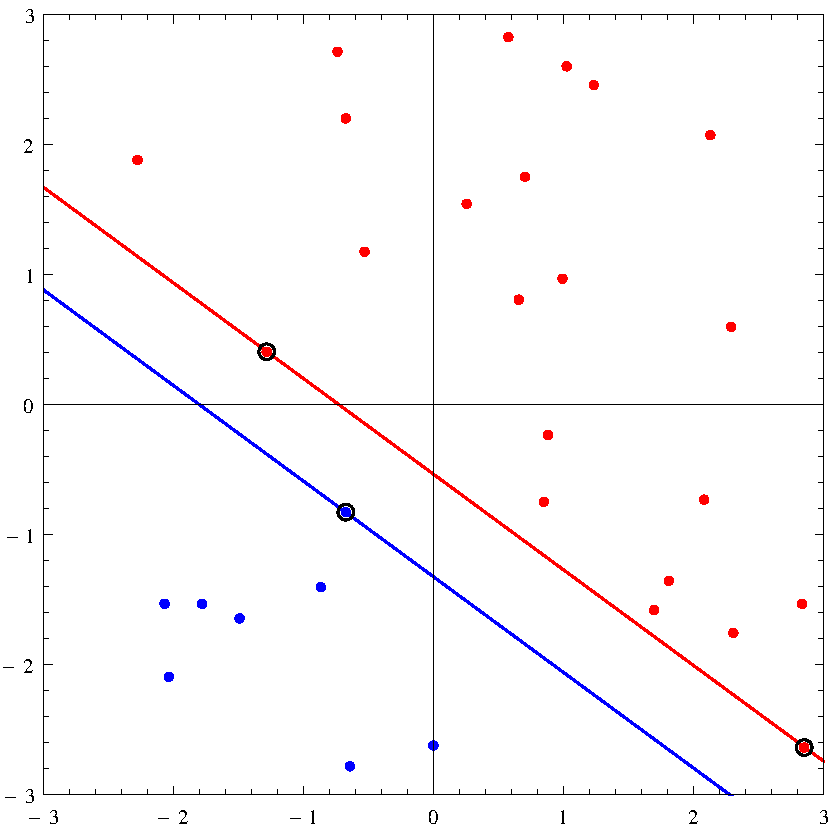
\includegraphics[scale=.55]{figures/math_lin_b}}
	\par}
\end{frame}

%%%%%%%%%%%%%%%%%%%%%%%%%%%%%%%%%%
%% Nonlinear case
%%%%%%%%%%%%%%%%%%%%%%%%%%%%%%%%%%
\section{Nonlinear case}
\label{sec:nonlinear_case}

<%= rex(slide,slides) %>
<% slide += 1 %>
\begin{frame}[c]\frametitle{What to do if linear separation is not possible?}
	\begin{itemize}
		\item We wish to map our data $x_i \in \mathbb{R}^d$ to some -- \emph{real} -- Hilbert space $\mathscr{H}$ with inner product $\langle \cdot,\cdot \rangle$,
			\[
				\Phi: \mathbb{R}^d \to \mathscr{H}.
			\]
		\vfill
		\item Wolfe dual problem involves only inner products $x_i \cdot x_j$ in $\mathbb{R}^d$.
		\vfill\pause
		\item Instead of those products we will have to compute expressions of the form
			\[
				K(x_i,x_j) := \langle \Phi(x_i), \Phi(x_j) \rangle, \quad K : \mathbb{R}^d \times \mathbb{R}^d \to \mathbb{R}.
			\]
		\vfill\pause
		\item N.B.:
			\begin{align*}
				K(u,v) &= K(v,u), & &u,v \in\mathbb{R}^d \\
				\sum_{i,j=1}^n \! c_i c_j K(u_i,u_j) &= \bigg\| \sum_{i=1}^n c_i \Phi(u_i) \bigg\|^2 \geq 0, & &n\in\mathbb{N}, \, u_i \in \mathbb{R}^d, \,c\in\mathbb{R}^n.
			\end{align*}
	\end{itemize}
\end{frame}

<%= rex(slide,slides) %>
<% slide += 1 %>
\begin{frame}[c]\frametitle{Kernel}
	\begin{block}{Definition}
		Any $K: X \times X \to \mathbb{R}$ such that
		\begin{itemize}
			\item $K(x,y) = K(y,x)$ for any $x,y \in X$,
			\item $K$ is positive definite, i.e. for any $n \geq 1$, $x_1,\ldots,x_n \in X$ and any $c_1,\ldots,c_n \in \mathbb{R}$
			\[
				\sum_{i,j=1}^n c_i c_j K(x_i,x_j) \geq 0.
			\]
		\end{itemize}
		is called \emph{kernel} on $X \times X$.
	\end{block}
	\vfill
	\begin{itemize}
		\item Application to SVM [Boser, Guyon and Vapnik, 1992].
	\end{itemize}
\end{frame}

<%= rex(slide,slides) %>
<% slide += 1 %>
\begin{frame}[c]\frametitle{On the other hand\ldots}
	\begin{itemize}
		\item \ldots one can start with a kernel $K: X \times X \to \mathbb{R}$ and ask whether there is a Hilbert space $\mathscr{H}$ and $\Phi: X \to \mathscr{H}$ such that
		\[
			K(x,y) = \langle \Phi(x), \Phi(y) \rangle, \quad x,y \in X.
		\]
		In this case it would be possible to use $K$ only.
		\vfill
		\item The answer to that question is positive.
	\end{itemize}
\end{frame}

<%= rex(slide,slides) %>
<% slide += 1 %>
\begin{frame}[c]\frametitle{RKHS}
	\begin{block}{Theorem}
		Let $X$ be a separable metric space and $K: X \times X \to \mathbb{R}$ a continuous kernel on $X \times X$. Then there is a separable Hilbert space $\mathscr{H}$ of functions on $X$ and mapping $\Phi: X \to \ell^2 \simeq \mathscr{H}$ such that
		\[
			K(u,v) = \langle \Phi(u), \Phi(v) \rangle_{\ell^2}, \quad u,v\in X.
		\]
	\end{block}
	\vfill
	\begin{block}{Note}
		$\mathscr{H}$ is the \emph{Reproducing kernel Hilbert space} (RKHS) associated with $K$. This terminology is due to the property
		\[
			f(x) = \langle K_x, f \rangle, \quad x\in X, \, f\in \mathscr{H},
		\]
		where $K_x = K(x,\cdot)$.
	\end{block}
\end{frame}

<%= rex(slide,slides) %>
<% slide += 1 %>
\begin{frame}[t]\frametitle{Proof}
	\begin{itemize}
		\item $V := \spn_\mathbb{R} \{ K_x \,:\, x\in X \}$, recall $K_x(y) = K(x,y)$.
		\pause
		\item For $f,g \in V$, $f = \sum_{i=1}^n c_i K_{x_i}$, $g = \sum_{j=1}^m d_j K_{y_j}$ set
			\[
				\langle f,g \rangle := \sum_{i,j} c_i d_j K(x_i,x_j) = \sum_i c_i g(x_i) = \sum_j d_j f(x_j).
			\]
			$\langle\cdot,\cdot\rangle$ does not depend on the representation of $f$ and $g$, is bilinear, symmetric and $\langle f,f \rangle \geq 0$ for any $f\in V$.
		\pause
		\item $\langle\cdot,\cdot\rangle$ has the reproducing property,
			\[
				\langle f,K_x \rangle = \sum_{j=1}^1 1\cdot f(x) = f(x), \quad f\in V, x\in X.
			\]
		\pause
		\item
			Since
			\[
				f(x)^2 = \langle f, K_x \rangle^2 \leq \langle f,f \rangle \cdot \langle K_x, K_x \rangle = \|f\|^2 \cdot K(x,x), \quad x\in X,
			\]
			we conclude that if $\|f\| = 0$ then $f(x) = 0$ for any $x\in X$.
	\end{itemize}
\end{frame}

<%= rex(slide,slides) %>
<% slide += 1 %>
\begin{frame}[t]\frametitle{Proof (cont'd)}
	\begin{itemize}
		\item The pair $(V,\langle\cdot,\cdot\rangle)$ forms a real pre-Hilbert space.
		\pause
		\vfill
		\item Let $\mathscr{H}$ be the completion of $(V,\langle\cdot,\cdot\rangle)$.
		\pause
		\vfill
		\item Note that if $\{f_n\}_{n=1}^\infty$ is a Cauchy sequence in $V$ then $\{f_n(x)\}_{n=1}^\infty$ is a Cauchy sequence in $\mathbb{R}$ for any $x\in\mathbb{R}$. Indeed, recall the inequality
		\[
			(f_n(x) - f_m(x))^2 \leq \|f_n - f_m\|^2 \cdot K(x,x).
		\]
		So $\mathscr{H}$ consists of a larger class of real valued functions on $X$.
		\pause
		\vfill
		\item $\mathscr{H}$ has the reproducing property and is separable.
	\end{itemize}
\end{frame}

<%= rex(slide,slides) %>
<% slide += 1 %>
\begin{frame}[c]\frametitle{Proof (cont'd)}
	\begin{itemize}
		\item Let $\{\phi_i\}_{i}$ be an orthonormal basis of $\mathscr{H}$. For any $x\in X$ we have the Fourier expansion of $K_x \in V \subset \mathscr{H}$
		\[
			K_x = \sum_{i} \langle \phi_i, K_x \rangle \phi_i.
		\]
		For any $y \in X$ we obtain
		\[
			K(x,y) = K_x(y) = \sum_{i} \phi_i(x) \phi_i(y).
		\]
		So $\Phi: X \to l^2(\mathbb{N},\mathbb{R})$, $\Phi(x) := \{\phi_i(x)\}_i$ \hfill\qedsymbol
	\end{itemize}
\end{frame}

<%= rex(slide,slides) %>
<% slide += 1 %>
\begin{frame}[t]\frametitle{Problem to be maximized}  
	\begin{block}{Wolfe dual with the Kernel}
		Maximize
		\[
			\sum_{i=1}^\ell \lambda_i -\frac{1}{2} \sum_{i,j=1}^\ell \lambda_i \lambda_j y_i y_j K(x_i,x_j)
		\]
		with respect to $\lambda \geq 0$ subject to $\sum_{i=1}^\ell \lambda_i y_i = 0$.
	\end{block}
	\begin{block}{Classificator}
		Compute the sign of
		\[
			w\cdot x + b = \sum_{x_i \, \text{is s.v.}} \lambda_i y_i x_i \cdot x + b \leftrightarrow \sum_{x_i \, \text{is s.v.}} \lambda_i y_i K(x_i,x) + b,
		\]
		where
		\[
			b = \frac{1}{y_i} - w \cdot x_i = y_i - \sum_{x_j \, \text{is s.v.}} \lambda_j y_j x_j \cdot x_i \leftrightarrow y_i - \sum_{x_j \, \text{is s.v.}} \lambda_j y_j K(x_j,x_i).
		\]
	\end{block}
\end{frame}

<%= rex(slide,slides) %>
<% slide += 1 %>
\begin{frame}[c]\frametitle{Example}
	{\centering
	\only<1>{
		Results for "radial basis kernel"
		\[
			K(u,v) = \exp \big( \!-\!\| u - v \|^2 \,/\, (2\sigma^2) \big), \quad u,v\in\mathbb{R}^d.
		\]
	}
	\only<2>{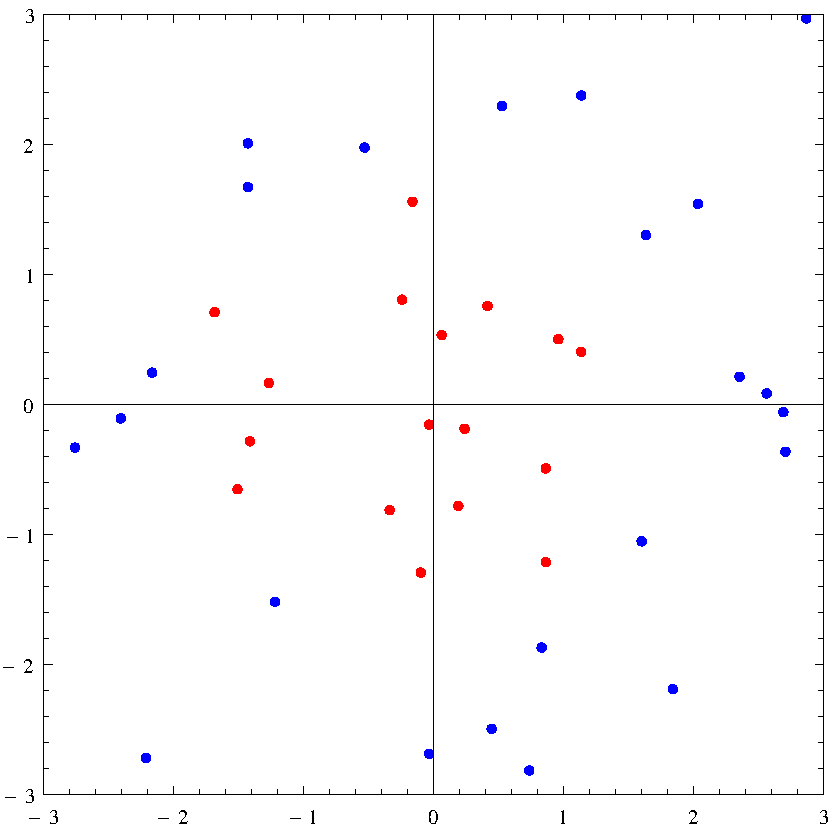
\includegraphics[scale=.55]{figures/math_non_lin_a}}
	\only<3>{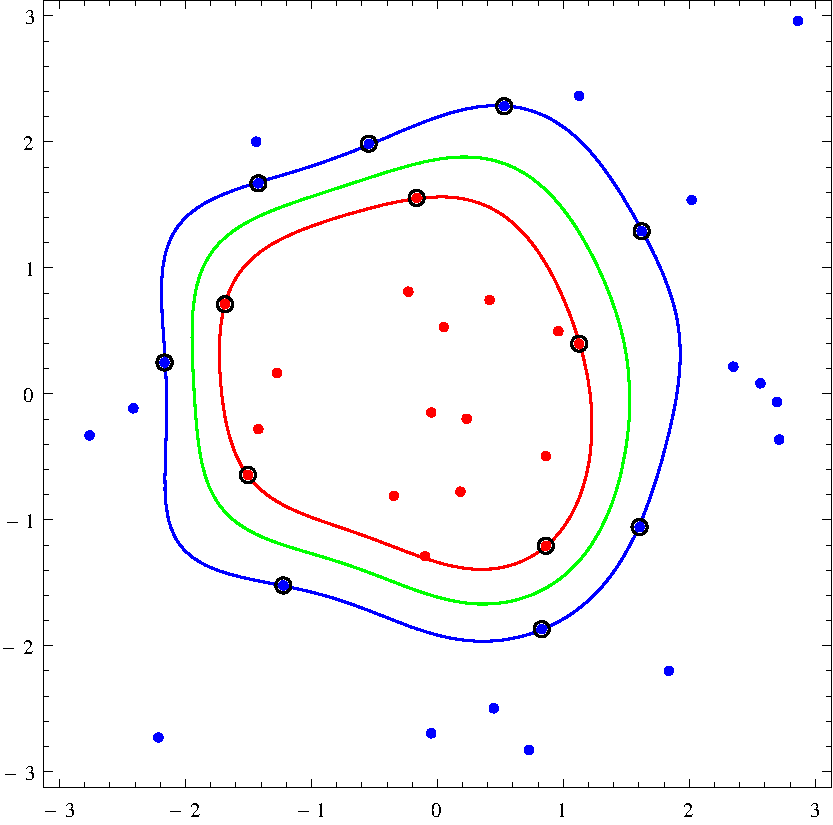
\includegraphics[scale=.55]{figures/math_non_lin_b}}
	\par}
\end{frame}

<%= rex(slide,slides) %>
<% slide += 1 %>
\begin{frame}[c]\frametitle{Example}
	{\centering
	\only<1>{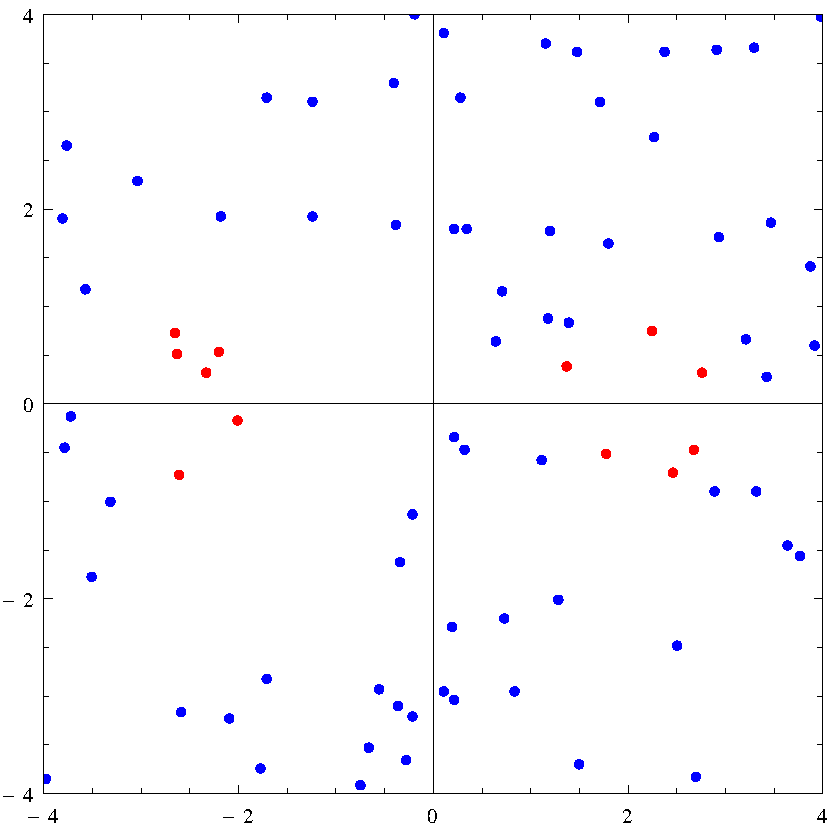
\includegraphics[scale=.55]{figures/math_non_lin_a_b}}
	\only<2>{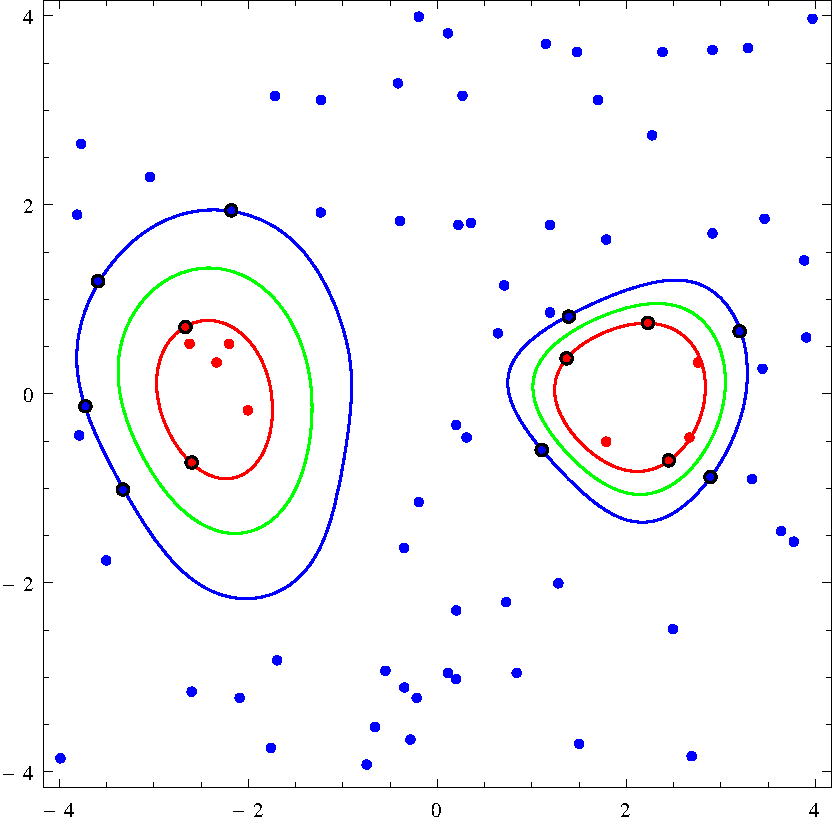
\includegraphics[scale=.55]{figures/math_non_lin_b_b}}
	\par}
\end{frame}

<%= rex(slide,slides) %>
<% slide += 1 %>
\begin{frame}[c]\frametitle{Example}
	{\centering
		\includegraphics[scale=.44]{figures/learning}
	\par}
\end{frame}

<%= rex(slide,slides) %>
<% slide += 1 %>
\begin{frame}[c]{}

	{\centering\Large\bfseries Thank you for your attention.\par}
	
\end{frame}

\end{document}